%\documentclass{article}
\documentclass[twoside,slovak, a4paper]{article}
\usepackage{graphicx} % Required for inserting images
\usepackage{geometry} % Required for customizing page layout
\usepackage[slovak]{babel}
\usepackage{url} 
\usepackage{hyperref}
\usepackage{subcaption} % Include the subcaption package
\usepackage{multirow}
\usepackage{xcolor}
\usepackage{tikz}



\usepackage{fancyhdr} % Required for custom headers and footers
\pagestyle{fancy}
\fancyhf{}
\fancyfoot[R]{\thepage} % Page number on the right side of the footer

\renewcommand{\headrulewidth}{0pt} % Remove the horizontal line in the header

\newcommand\blankpage{
    \null
    \thispagestyle{empty}
    \addtocounter{page}{1}
    \newpage}


\newcommand\blankpag{%
    \clearpage
    \vspace*{\fill}
   
}

\begin{document}
% Define the title page
\begin{titlepage}
\newgeometry{left=1in, right=1in} % Adjust margins as needed

\begin{center}

% Upper Section
{\Large
Slovenská technická univerzita v Bratislave \\
Fakulta informatiky a informačných technológií \\

\vspace{0.4cm}

FIIT-XXXX-XXXXX

\vspace{5cm}

Filip Mojto \\

}

%\vspace{1cm} % Space between upper and middle section

% Middle Section
{\Large
%Filip Mojto \\

\vspace{0.8cm}
POUŽITIE JEDNODUCHEJ AUTOMATIZÁCIE\\
ZA ÚČELOM ZJEDNODUŠENIA\\
KAŽDODENNÝCH RUTINNÝCH ČINNOSTÍ \\
\vspace{0.8cm}
}

{\Large
Bakalárska práca \\
}


\vspace{1cm} % Space between middle and lower section
\vfill
% Lower Section
\begin{flushleft}
%\newcommand{\myindent}{\hspace*{0.01em}}\t
\begin{tabular}{@{}ll}
Študijný program: & Informatika \\
Študijný odbor:  & Informatika \\
Miesto vypracovania: & Ústav počítačového inžinierstva a aplikovanej informatiky \\
Vedúci práce: & Mgr. Andrej Uhrín \\
Ďalší vedúci: & Ing. Katarína Jelemenská PhD. \\
\end{tabular}
\\
\vspace{0.7cm}
Máj 2024
%\end{tabular}
%\end{tabular}{@{}ll}
\end{flushleft}
\vspace*{-2cm} % Adjust the value as needed

\end{center}

\restoregeometry % Restore the default margins

\end{titlepage}


\blankpage

% \geometry{left=2.5cm, right=2.5cm, top=2.5cm, bottom=2.5cm} % Set custom margins

\definecolor{color_283006}{rgb}{1,1,1}
\definecolor{color_29791}{rgb}{0,0,0}
\begin{tikzpicture}[overlay]
\path(0pt,0pt);
\filldraw[color_283006][even odd rule]
(57pt, -183.85pt) -- (524.95pt, -183.85pt)
 -- (524.95pt, -183.85pt)
 -- (524.95pt, -62pt)
 -- (524.95pt, -62pt)
 -- (57pt, -62pt) -- cycle
;
\filldraw[color_283006][even odd rule]
(57pt, -227.05pt) -- (524.95pt, -227.05pt)
 -- (524.95pt, -227.05pt)
 -- (524.95pt, -183.9pt)
 -- (524.95pt, -183.9pt)
 -- (57pt, -183.9pt) -- cycle
;
\filldraw[color_283006][even odd rule]
(57pt, -699.75pt) -- (524.95pt, -699.75pt)
 -- (524.95pt, -699.75pt)
 -- (524.95pt, -227.1pt)
 -- (524.95pt, -227.1pt)
 -- (57pt, -227.1pt) -- cycle
;
\filldraw[color_283006][even odd rule]
(57pt, -183.85pt) -- (524.95pt, -183.85pt)
 -- (524.95pt, -183.85pt)
 -- (524.95pt, -62pt)
 -- (524.95pt, -62pt)
 -- (57pt, -62pt) -- cycle
;
\filldraw[color_283006][even odd rule]
(57pt, -227.05pt) -- (524.95pt, -227.05pt)
 -- (524.95pt, -227.05pt)
 -- (524.95pt, -183.9pt)
 -- (524.95pt, -183.9pt)
 -- (57pt, -183.9pt) -- cycle
;
\filldraw[color_283006][even odd rule]
(57pt, -699.75pt) -- (524.95pt, -699.75pt)
 -- (524.95pt, -699.75pt)
 -- (524.95pt, -227.1pt)
 -- (524.95pt, -227.1pt)
 -- (57pt, -227.1pt) -- cycle
;
\end{tikzpicture}
\begin{picture}(-5,0)(2.5,0)
\put(0,0){\fontsize{12}{1}\usefont{T1}{ptm}{m}{n}\selectfont\color{color_29791} }
\put(-55,0){\fontsize{12}{1}\usefont{T1}{ptm}{b}{n}\selectfont\color{color_29791}Slovenská technická univerzita v Bratislave}

\put(-55,-14){\fontsize{12}{1}\usefont{T1}{ptm}{b}{n}\selectfont\color{color_29791}Ústav počítačového inžinierstva a aplikovanej}
\put(-55,-28){\fontsize{12}{1}\usefont{T1}{ptm}{b}{n}\selectfont\color{color_29791}informatiky}
\put(298.4,-100.8){\fontsize{12}{1}\usefont{T1}{ptm}{m}{n}\selectfont\color{color_29791} }
\put(235.9,0){\fontsize{12}{1}\usefont{T1}{ptm}{b}{n}\selectfont\color{color_29791}Fakulta informatiky a informačných}
\put(235.9,-14){\fontsize{12}{1}\usefont{T1}{ptm}{b}{n}\selectfont\color{color_29791} technológií}

\put(235.9,-28){\fontsize{12}{1}\usefont{T1}{ptm}{b}{n}\selectfont\color{color_29791}2023/2024}

\put(58.6,-128.4){\fontsize{12}{1}\usefont{T1}{ptm}{m}{n}\selectfont\color{color_29791} }
\put(58.6,-142.2){\fontsize{12}{1}\usefont{T1}{ptm}{m}{n}\selectfont\color{color_29791} }
\put(135,-115.75){
\includegraphics[width=105pt,height=39pt]{latexImage_f6190465bc5b3282313af98a57247f32.png}}
\put(75.2,-175.3){\fontsize{13.5}{1}\usefont{T1}{ptm}{b}{n}\selectfont\color{color_29791}ZADANIE BAKALÁRSKEJ PRÁCE}
\put(-58,-204.4){\fontsize{12}{1}\usefont{T1}{ptm}{m}{n}\selectfont\color{color_29791} }
\put(-58,-218.3){\fontsize{12}{1}\usefont{T1}{ptm}{m}{n}\selectfont\color{color_29791}Autor práce:}
\put(87.5,-218.3){\fontsize{12}{1}\usefont{T1}{ptm}{m}{n}\selectfont\color{color_29791}Filip Mojto}
\put(-58,-232.1){\fontsize{12}{1}\usefont{T1}{ptm}{m}{n}\selectfont\color{color_29791}Študijný program:}
\put(87.5,-232.1){\fontsize{12}{1}\usefont{T1}{ptm}{m}{n}\selectfont\color{color_29791}informatika}
\put(-58,-245.9){\fontsize{12}{1}\usefont{T1}{ptm}{m}{n}\selectfont\color{color_29791}Študijný odbor:}
\put(87.5,-245.9){\fontsize{12}{1}\usefont{T1}{ptm}{m}{n}\selectfont\color{color_29791}informatika}
\put(-58,-259.7){\fontsize{12}{1}\usefont{T1}{ptm}{m}{n}\selectfont\color{color_29791}Evidenčné číslo:}
\put(87.5,-259.7){\fontsize{12}{1}\usefont{T1}{ptm}{m}{n}\selectfont\color{color_29791}FIIT-16768-116253}
\put(-58,-273.5){\fontsize{12}{1}\usefont{T1}{ptm}{m}{n}\selectfont\color{color_29791}ID študenta:}
\put(87.5,-273.5){\fontsize{12}{1}\usefont{T1}{ptm}{m}{n}\selectfont\color{color_29791}116253}
\put(-58,-287.3){\fontsize{12}{1}\usefont{T1}{ptm}{m}{n}\selectfont\color{color_29791}Vedúci práce:}
\put(87.5,-287.3){\fontsize{12}{1}\usefont{T1}{ptm}{m}{n}\selectfont\color{color_29791}Mgr. Andrej Uhrin}
\put(-58,-301.1){\fontsize{12}{1}\usefont{T1}{ptm}{m}{n}\selectfont\color{color_29791}Vedúci pracoviska:}
\put(87.5,-301.1){\fontsize{12}{1}\usefont{T1}{ptm}{m}{n}\selectfont\color{color_29791}Ing. Katarína Jelemenská, PhD.}
\put(-58,-314.9){\fontsize{12}{1}\usefont{T1}{ptm}{m}{n}\selectfont\color{color_29791} }
\put(87.5,-314.9){\fontsize{12}{1}\usefont{T1}{ptm}{m}{n}\selectfont\color{color_29791} }
\put(-58,-328.7){\fontsize{12}{1}\usefont{T1}{ptm}{m}{n}\selectfont\color{color_29791}Názov práce:}
\put(87.5,-330.1){\fontsize{13.5}{1}\usefont{T1}{ptm}{b}{n}\selectfont\color{color_29791}Použitie jednoduchej automatizácie za účelom }
\put(87.5,-345.7){\fontsize{13.5}{1}\usefont{T1}{ptm}{b}{n}\selectfont\color{color_29791}zefektívnenia každodenných rutinných činností}
\put(-58,-359.8){\fontsize{12}{1}\usefont{T1}{ptm}{m}{n}\selectfont\color{color_29791} }
\put(87.5,-359.8){\fontsize{12}{1}\usefont{T1}{ptm}{m}{n}\selectfont\color{color_29791} }
\put(-58,-373.6){\fontsize{12}{1}\usefont{T1}{ptm}{m}{n}\selectfont\color{color_29791}Jazyk, v ktorom sa}
\put(177.6,-373.6){\fontsize{12}{1}\usefont{T1}{ptm}{m}{n}\selectfont\color{color_29791} }
\put(-58,-387.4){\fontsize{12}{1}\usefont{T1}{ptm}{m}{n}\selectfont\color{color_29791}práca vypracuje:}
\put(87.5,-373.6){\fontsize{12}{1}\usefont{T1}{ptm}{m}{n}\selectfont\color{color_29791}slovenský jazyk}

\put(-58,-405.2){\fontsize{12}{1}\usefont{T1}{ptm}{m}{n}\selectfont\color{color_29791} }
\put(87.5,-405.2){\fontsize{12}{1}\usefont{T1}{ptm}{m}{n}\selectfont\color{color_29791} }
\put(-58,-419){\fontsize{12}{1}\usefont{T1}{ptm}{m}{n}\selectfont\color{color_29791}Špecifikácia zadania:}

\put(87.5,-419){\fontsize{12}{1}\usefont{T1}{ptm}{m}{n}\selectfont\color{color_29791}Automatizácia predstavuje jednu z nádejí aktuálnej doby }

\put(87.5,-432.8){\fontsize{12}{1}\usefont{T1}{ptm}{m}{n}\selectfont\color{color_29791}ponúkajúcich možnosti zvýšiť kvalitu a množstvo dodanej práce.}

\put(87.5,-446.6){\fontsize{12}{1}\usefont{T1}{ptm}{m}{n}\selectfont\color{color_29791}Napriek tomu jej plný potenciál sa nedarí dosiahnuť väčšine }

\put(87.5,-460.4){\fontsize{12}{1}\usefont{T1}{ptm}{m}{n}\selectfont\color{color_29791}technologických firiem. Identifikácia spôsobov a implementácia }

\put(87.5,-474.2){\fontsize{12}{1}\usefont{T1}{ptm}{m}{n}\selectfont\color{color_29791}jednoduchej automatizácie na úrovni jednotlivca ponúka možnosť }

\put(87.5,-488){\fontsize{12}{1}\usefont{T1}{ptm}{m}{n}\selectfont\color{color_29791}ako pochopiť problémy a ponúknuť riešenia k využitiu potenciálu }

\put(87.5,-501.8){\fontsize{12}{1}\usefont{T1}{ptm}{m}{n}\selectfont\color{color_29791}automatizácie. Analyzujte činnosti vhodné na automatizáciu a ich }

\put(87.5,-515.6){\fontsize{12}{1}\usefont{T1}{ptm}{m}{n}\selectfont\color{color_29791}potenciál - dopad automatizácie na prácu jednotlivca. Pre väčší }

\put(87.5,-529.4){\fontsize{12}{1}\usefont{T1}{ptm}{m}{n}\selectfont\color{color_29791}prínos práce zvoľte činnosti dobre známe širokému spektru ľudí - }

\put(87.5,-543.2){\fontsize{12}{1}\usefont{T1}{ptm}{m}{n}\selectfont\color{color_29791}napr. automatizácia procesu objednávania jedla podľa kalendára }

\put(87.5,-557){\fontsize{12}{1}\usefont{T1}{ptm}{m}{n}\selectfont\color{color_29791}(počet osôb, čas, adresa, preferencie na typ kuchyne a pod.). Na }

\put(87.5,-570.8){\fontsize{12}{1}\usefont{T1}{ptm}{m}{n}\selectfont\color{color_29791}základe analýzy vyberte vhodný proces na automatizáciu. Navrhnite }

\put(87.5,-584.6){\fontsize{12}{1}\usefont{T1}{ptm}{m}{n}\selectfont\color{color_29791}spôsob automatizácie vybraného procesu a návrh implementujte vo }

\put(87.5,-598.4){\fontsize{12}{1}\usefont{T1}{ptm}{m}{n}\selectfont\color{color_29791}forme robota (softvéru), ktorý bude bežať na základe dohodnutých }

\put(87.5,-612.2){\fontsize{12}{1}\usefont{T1}{ptm}{m}{n}\selectfont\color{color_29791}podmienok (triggers) automaticky. Otestujte a zhodnoťte prínos }

\put(87.5,-626){\fontsize{12}{1}\usefont{T1}{ptm}{m}{n}\selectfont\color{color_29791}automatizácie k efektivite práce pracovníka, dopad na kvalitu }

\put(87.5,-639.8){\fontsize{12}{1}\usefont{T1}{ptm}{m}{n}\selectfont\color{color_29791}a kvantitu. Identifikujte prípadné problémy, spojené }

\put(87.5,-653.6){\fontsize{12}{1}\usefont{T1}{ptm}{m}{n}\selectfont\color{color_29791}s automatizáciou.}

\put(-58,-667.4){\fontsize{12}{1}\usefont{T1}{ptm}{m}{n}\selectfont\color{color_29791} }
\put(87.5,-667.4){\fontsize{12}{1}\usefont{T1}{ptm}{m}{n}\selectfont\color{color_29791} }

\end{picture}
\newpage
\begin{tikzpicture}[overlay]
\path(0pt,0pt);
\filldraw[color_283006][even odd rule]
(57pt, -160.15pt) -- (524.95pt, -160.15pt)
 -- (524.95pt, -160.15pt)
 -- (524.95pt, -62pt)
 -- (524.95pt, -62pt)
 -- (57pt, -62pt) -- cycle
;
\filldraw[color_283006][even odd rule]
(57pt, -160.15pt) -- (524.95pt, -160.15pt)
 -- (524.95pt, -160.15pt)
 -- (524.95pt, -62pt)
 -- (524.95pt, -62pt)
 -- (57pt, -62pt) -- cycle
;
\end{tikzpicture}
\begin{picture}(-5,0)(2.5,0)

\put(-58,0){\fontsize{12}{1}\usefont{T1}{ptm}{m}{n}\selectfont\color{color_29791}Rozsah práce: }

\put(87.5,-0){\fontsize{12}{1}\usefont{T1}{ptm}{m}{n}\selectfont\color{color_29791}40}
\put(-58,-24){\fontsize{12}{1}\usefont{T1}{ptm}{m}{n}\selectfont\color{color_29791}Termín odovzdania práce: }
\put(87.5,-24){\fontsize{12}{1}\usefont{T1}{ptm}{m}{n}\selectfont\color{color_29791}21.05.2024}



\put(-58,-48){\fontsize{12}{1}\usefont{T1}{ptm}{m}{n}\selectfont\color{color_29791}Dátum schválenia zadania}
\put(-58,-62){\fontsize{12}{1}\usefont{T1}{ptm}{m}{n}\selectfont\color{color_29791}práce:}

\put(-58,-86){\fontsize{12}{1}\usefont{T1}{ptm}{m}{n}\selectfont\color{color_29791}Zadanie práce schválil:}

\end{picture}



\blankpage

\blankpage

\null
\vfill

\noindent
Čestne prehlasujem, že som túto prácu vypracoval samostatne, na základe konzultácií a s použitím uvedenej literatúry.

\vspace*{0.8cm}

\noindent
V Bratislave, 15.5.2023

\vspace*{0cm}

\begin{flushright}

Filip Mojto \hspace*{1cm}

\vspace*{-0.5cm}

\end{flushright}

\newpage

\blankpage

Tu moze byt podakovanie

\blankpage

\blankpage

\section*{Anotácia}

\vspace*{0.3cm}

Slovenská technická univerzita v Bratislave\\

\noindent
FAKULTA INFORMATIKY A INFORMAČNÝCH TECHNOLÓGIÍ\\[0.2em]

\noindent
\begin{tabular}{@{}ll}
Študijný program: \hspace{11em} & Informatika \\[3em]
Autor: \hspace{11em} & Filip Mojto \\[0.7em]
Bakalárska práca: \hspace{11em} & Použitie jednoduchej automatizácie \\
 \hspace{11em} & za účelom zjednodušenia \\
 \hspace{11em} & každodenných rutinných činností\\[0.7em]
Vedúci bakalárskej práce: \hspace{11em} & Mgr. Andrej Uhrín\\[0.7em]
Ďalší vedúci: \hspace{11em} & Ing. Katarína Jelemenská PhD.\\[1.7em]

\end{tabular}

\noindent
Máj 2024\\[2em]

\noindent
Tento dokument sa venoval komplexnej analýze automatizácie v hardvérovej i softvérovej podobe. Hlavným cieľom bolo získať jasný prehľad o stave automatizácie v súčasnosti, potom sa sústrediť na zvolený prípad. Po dôkladnej analýze práca navrhovala a implementovala jednoduchú automatizáciu sústreďujúcu sa na vybraný prípad v oblasti automatizácie. Prvá kapitola úvodom prehľadne zasväcuje čitateľa do skúmanej problematiky automatizácie, neskôr sa venuje významným témam a ich vplyvom na automatizáciu ako napríklad umelá inteligencia. Kapitola sa snažila najskôr poskytnúť všeobecný prehľad o problematike, neskôr sa viac konkretizovala na významné pod-oblasti ako roboty, automatizácie realizované počítačom a hardvérom a na záver skúmala stav automatizácie založenej na softvéri. Druhá kapitola sa viac orientovala na nami zvolený prípad - virtuálny obchod, kde hlavným cieľom bolo získať prehľad o stave automatizácie vo virtuálnom obchode, analyzovať rôzne príklady a zistiť tak možné nedostatky, ktoré by bolo možné zautomatizovať. Posledná kapitola realizovala softvérovú automatizáciu vo forme programu, ktorá sa špecializovala na zvolený prípad a ponúkla tak zaujímavé riešenie v skúmanej oblasti.


\blankpage

\blankpage


\section*{Annotation}

\vspace*{0.3cm}

Slovak University of Technology Bratislava\\

\noindent
FACULTY OF INFORMATICS AND INFORMATION TECHNOLOGIES\\[0.2em]

\noindent
\begin{tabular}{@{}ll}
Degree course: \hspace{11em} & Informatics \\[3em]
Author: \hspace{11em} & Filip Mojto \\[0.7em]
Bachelor's Thesis: \hspace{11em} & The use of simple automation \\
 \hspace{11em} & for the purpose of \\
 \hspace{11em} & streamlining everyday routine tasks\\[0.7em]
Supervisor: \hspace{11em} & Mgr. Andrej Uhrín\\[0.7em]
Additional advisor: \hspace{11em} & Ing. Katarína Jelemenská\\[1.7em]
\end{tabular}

\noindent
May 2024\\[2em]

\noindent
This document focused on a comprehensive analysis of automation in both hardware and software forms. The main objective was to gain a clear overview of the current state of automation and then concentrate on a chosen case. After a thorough analysis, the work proposed and implemented a simple automation focusing on the selected case in the field of automation. The first chapter begins with a clear introduction, providing the reader with an overview of the studied issue of automation. It later delves into significant topics and their impact on automation, such as artificial intelligence. The chapter initially aimed to offer a general overview of the problem, later becoming more specific in exploring important sub-areas like robots, computer and hardware-based automation, and finally examining the state of software-based automation. The second chapter was more oriented towards the chosen case – a virtual store. The primary goal was to obtain an overview of the state of automation in virtual stores, analyze various examples, and identify potential shortcomings that could be automated. The final chapter implemented software automation in the form of a program, specializing in the chosen case and providing an interesting solution in the studied area.

\blankpage

\blankpage

\tableofcontents

\pagenumbering{roman}
\setcounter{page}{11}
\blankpag
\blankpage
\pagenumbering{arabic}
\setcounter{page}{1}
\section{Úvod}

\blankpag\blankpage

\section{Automatizácia}

Začnime stručným úvodom do problematiky. Nakoľko sa v našej práci sa primárne venujeme procesu automatizácie, je vhodné najskôr zo všeobecnejšieho pohľadu ozrejmiť, čo vlastne pojem automatizácia znamená. \textbf{Automatizácia} pochádza z anglického výrazu 'automation' (niekedy aj 'automatization') a znamená zjednodušenie a zefektívnenie vykonávania manuálnych úloh alebo činností, a to aj za účelom zvýšenia presnosti. \cite{AH:WAS}. Automatizácia už dávno prekročila svoje korene spočívajúce vo výrobe a rozšírilia ich na mnohé ďalšie uplatnenia, či už v zdravotníctve, bezpečnosti, doprave, poľnohospodárstve, v budovaní alebo v energetike a v mnohých ďalších oblastiach. Vývoj v oblasti automatizácie kladie dôraz na efektívnosť, produktivitu, výslednú kvalitu a spoľahlivosť spoliehajúc na systémy, ktoré operujú autonómne, často v štrukturovaných prostrediach a na dlhšiu dobu a na explicitné usporiadanie takýchto prostredí. Toto tvrdenie dáva do popredia akýsi dôraz, ktorý automatizácia kladie buď viac na dokonalejšiu štruktúru, a teda na spoľahlivosť, alebo preferuje menej štruktúrované prostredia, kde má zase väčšiu prispôsobivosť. \cite{IEEE2012} Ešte uvádzame jeden, tentokrát strúčnejší výrok, ktorý tvrdí, že automatizácia je mocná, má obrovský a obvivuhodný vplyv na civilizáciu, na ľudstvo, avšak môže prinášať i riziká.\cite{Nof2009}

Ďalším dôležitým pojmom v oblasti automatizácie je \textbf{robot} alebo \textbf{automat} (z ang. Automaton). Robot je autonómne zariadenie, ktoré je závislé na nejakom zdroje energie a môže vykonávať komplexné série akcií bez nutnosti ľudského zásahu ako odpoved na programy alebo rôzne externé stimuly. Robot definuje autonómne zariadenie alebo nástroj, nezahŕňa však také platformy ako infraštruktúra či rôzne inštalácie alebo ďalšie automatické systémy ako ako automatizačný softvér.\cite{Nof2009}

\subsection*{Stručný formalizmus}

V tejto časti stručne načrtneme, akú má komplexný proces automatizácie štruktúru. Tú možno vidieť na obrázku 1. Presne sa tu vymedzujú možné vlastnosti typické pre akúkoľvek automatizáciu. Ide o akúsi konfiguráciu, ktorá charakterizuje akéhokoľvek robota alebo inú platformu.

\begin{figure}[tbh]
  \centering
  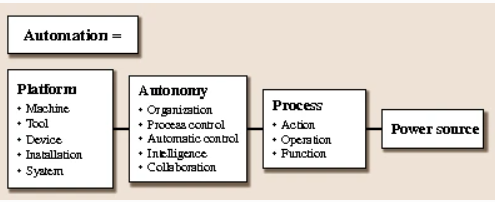
\includegraphics[width=0.7\textwidth]{pics/automation_strct.png}
  \caption{Základná štruktúra automatizácie\cite{Nof2009}}
  \label{fig:1}
\end{figure}



Každá automatizácia musí fungovať na nejakej \textbf{platforme} alebo na \textbf{systéme platforiem}. Či už je to zariadenie, inštalácia alebo systém. 
\textbf{Autonómia} predstavuje samostatnú, zautomatizovanú oblasť, ktorú automatizácia zahŕňa a charakterizuje jej komplexnú funkcionalitu. Napríklad pre UI by bola autonómia inteligencia. Čo daná automatizácia vykonáva, to popisuje jej \textbf{proces}, napríklad môže vykonať nejakú akciu, či už poslať mail alebo plánovať rutinné zálohovanie dát. Automatizácie vykonávajú vo veľa prípadoch aj rôzne operácie, napríklad v oblasti výroby, ktoré boli kedysi vykonávané ľudskou manuálnou prácou. Alebo môže ísť o vykonávanie funkcií, napríklad softvér vykonáva pomocou algoritmov rôzne kalkulácie, atď.\cite{Nof2009}:

\subsection{Umelá inteligencia}

Ako vlastne súvisí umelá inteligencia s automatizáciou ? Najskôr stručný opis umelej inteligencie.

Umelá inteligencia (často pod skratkou AI) je schopnosť systému vnímať očakávané ale aj neočakávané, nové udalosti, rozhodovať aké akcie je nutné vykonať za týchto podmienok či okolností a náležite akcie plánovať. Hlavné oblasti umelej inteligencie sú systémy založené na zbere vedomostí, počítačové senzorické systémy, systémy na spracovanie jazyka a strojové učenie.\cite{Nof2009}

Umelá inteligencia je vlastne ľudská inteligencia implementovaná na stroje či zariadenia, a to hlavne skrz počítače a komunikáciu. Ide opäť o automatizáciu, takže AI dokáže fungovať sammostatne, bez ľudskej manipulácie počas jej fungovania a môže kombinovať inteligenciu viacerých ľudí a navyše aj zlepšiť vlastné schopnosti automatickým učením a adaptáciou. Dokáže byť automaticky distribuovaná, duplikovaná, zdieľaná, zdedená a v prípade nutnosti aj obmedzená či úplne odstránená. S príchodom týchto vlastností došlo prirodzene k ohromnému progresu v oblasti technológií.\cite{Nof2009}

Teraz uvedieme rozdielny pohľad tento jav, možno trocha negatívny. Častou konfrontovanou nevýhodou je zníženie pracovných miest a tým aj zvýšenie nezamestnanosti. Nahradí automatizácia v kombinácii s umelou inteligenciou bežných pracovníkov ? Jeden zdroj uvádza, že kým niektoré odhady v tomto pohľade sú menej pesimistické, určité kľúčové štúdie uviedli, že veľké množstvo pracovníkov príjde kvôli rýchlo sa rozvíjajúcej automatizácii v blízkej budúcnosti o prácu. Pohľad na tento trend je kontroverzný. Kým niektoré hypotézy hovoria o zlepšení práce, napríklad zvýšením autonómie, kreativite a slobode pracovníka, iné hovoria o zvýšení neistoty zachovania si pracovného pomeru.\cite{NAZARENO2021101679}


While some estimates are less striking, several key studies have estimated that large numbers of workers will find themselves out of a job or needing to make a major transition in the near future due to automation.

\subsection{Príklady automatizácie}

Teraz sa môžme ísť pozrieť na konkrétne prípady automatizácie v praxi. Existuje množstvo príkladov z rôznych oblastí, či už z oblasti robotiky alebo v oblasti softvéru.

\subsubsection*{Regulátor parnej turbíny}

Procesom je operácia parnej turbíny, ktorá automaticky riadi kompresor alebo generátor. Regulátor funguje na platforme zariadenia integrovaného systémom s kontrolérom programovateľnej logiky (PLC). Automanómia zahŕňa najmä automatickú aktiváciu či deaktiváciu a kontrolu rýchlosti turbíny, či programovateľné parametre regulátor pomocou obrazovky a mnohé ďalšie.\cite{Nof2009}

\subsubsection*{Spracovávanie digitálnych fotografií}

Platformou je v tomto prípade  softvérový systém. Process sú rôzne akcie editovania alebo vylepšovania fotografií, pridávania rôznych grafických prvkov, odstranovanie fľakov a dalšie procesy typické pre grafický editor. Autonómia predstavuje plne automatické funkcie hneď ako ich používateľ aktivuje. Softvér môže tieto akcie vykonávať semiautomaticky alebo aj ako zautomatizovanú sériu akcií.\cite{Nof2009}


\subsubsection*{Robotické striekanie náterov vozidiel}

Túto automatizáciu spravidla vykonávajú roboti, teda zariadenia a stroje. Okrem iného musia byť zahrnuté aj rôzne sensory, dopravný pás, sprejovacie vybavenie a integrácia s programovacím softvérom určenom na plánovanie akcií. Procesom je teda sprejovanie spolu s automatickým riadením pohybu auta, otváraním dverí a ďalšie. Autonómiu tvorí flexibilita pohybov, vyhýbanie sa kolíziám, koordinácia pásu, pohyb samotného robota, sprejovacie a striekacie operácie a ďalšie.

\begin{figure}
    \begin{subfigure}[t]{0.5\textwidth} % 0.5\textwidth makes each subfigure take up half the line
        \centering
          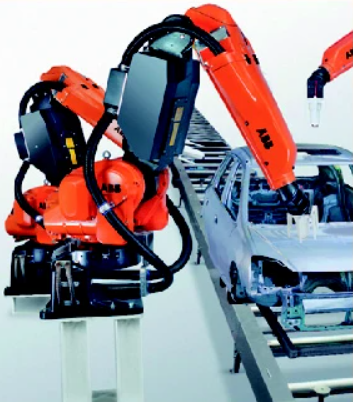
\includegraphics[width=0.6\textwidth]{pics/car_painting_automation.png}
          \caption{Automatické striekanie náterov vozidiel}
          \label{fig:2}
    \end{subfigure}
    \begin{subfigure}[t]{0.491\textwidth}
        \centering
        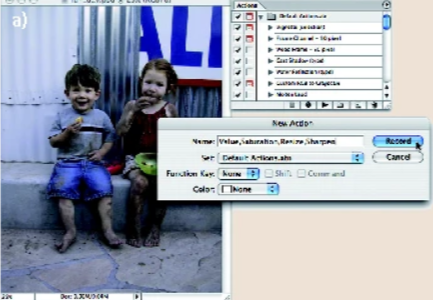
\includegraphics[width=1\linewidth]{pics/photo_edit_automation.png}
        \caption{Automatické editovania fotografií}
        \label{fig:3}
    \end{subfigure}
    \caption{Ilustrované prípady automatizácii v praxi\cite{Nof2009}}
\end{figure}

Teraz uvedieme ešte ďalšie prípady automatizácie, tentokrát formou tabuľky. Tá obsahuje zamerania rôznych štúdií a článkov v oblasti automatizácie. Pre 


\begin{table}[h]
    \centering
    \caption{Ďalšie prípady v oblasti automatizácie\cite{BAVARESCO2023100618}}
    \begin{tabular}{|c|c|c|c|c|c|} % Define the number of columns and their alignment
        \hline
        Autonómia & Prípad štúdie & Rok & SD & UE & UIA \\
        \hline\hline
        Automatizácia činností & Automatizácia spotrebičov & 2018 & áno & nie & nie \\
        \hline
        Automatizácia činností & Manažment IT žiadostí & 2018 & áno & nie & nie \\
        \hline
        \multirow{2}{*}{Manažement činností} & Manažement zamestnaneckých & \multirow{2}{*}{2018} & \multirow{2}{*}{áno} & \multirow{2}{*}{áno} & \multirow{2}{*}{áno}  \\ & činností & &&&\\
        \hline
        Architektúra Chatbot-a & Vládne služby & 2019 & nie & nie & nie \\
        \hline
        Automatizácia framework-ov & Analýza biznis dokumentu & 2019 & áno & nie & nie \\
        \hline
       Manažement činností & Plánovanie úloh pre zamestnancov & 2020 & áno & áno & áno \\
        \hline
    \end{tabular}
\end{table}

SD je skratka anglický výraz \textit{Service Deployed} a znamená to, či daná štúdia poskytla servic pre automatizáciu manuálnej práce zamestnancami. UE znamená \textit{Users Evaluation} a hovorí o tom, či bol výsledný produkt automatizácie hodnotený používateľmi. UIA je skratkou pre \textit{User Impact Analysis} a označuje, či bola vykonávaná nejaká analýza na dopad na užívateľov.


\subsection{Automatizácie založené na počítačoch}

Teraz, ked sme pochopili pojmu automatizáciu ako takej, môžeme sa teraz sústrediť viac na softvér. Najskôr si priblížime automatizačné systémy založené na počítačoch.

Osobné počítače sa v súčasnosti čoraz častejšie používajú na implementáciu časovo náročných úloh v (distribuovaných) automatizačných systémoch\cite{VITTURI2004145}. Tento trend výchadza z viacerých faktorov, napríklad:

\begin{itemize}
    \item Ohromný nárast počítačového výkonu
    \item Dostupnosť RTOS
    \item Vznik programovacích jazykov vhodných na kontrolné úlohy
    \item Narastajúce množstvo zariadení s rozhraním Fieldbus
\end{itemize}

Prvý faktor zaručuje, že v rovnakom stroji bude možnosť monitorovania či kontroly a súčasne aj možnosť vykonávanie úloh v reálnom čase. Druhý faktor umožňuje efektívne plánovanie úloh s tým, že kritické dostanú vyššie priority. Rozhranie Fieldbus umožňuje realizáciu distribuovaných architektúr s použitím hardvérových alebo softvérových produktov od rôznych výrobcov.\cite{VITTURI2004145}

\subsubsection*{Hardvérová štruktúra}

Na obrázku 5 možno vidieť najvšeobecnejší typ automatizačného systému založeného na PC. Možno vidieť, že osobný počítač, na ktorom prebiehajú automatizačné úlohy, komunikuje so strojovým zariadením skrz nejaký komunikačný systém.

\begin{figure}[tbh]
  \centering
  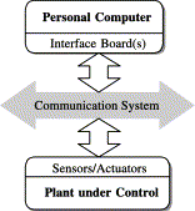
\includegraphics[width=0.4\textwidth]{pics/hardware_structure.png}
  \caption{Hardvérová štruktúra\cite{VITTURI2004145}}
  \label{fig:4}
\end{figure}

Tento typ rozhrania používaného počítačom je evidentne závislý na type komunikačného systému. V posledných rokoch bolo pripojenie ku stroju implementované väčšinou pomocou spojení implementovaných od jedného bodu k druhému, pričom každý koniec bol určený pre dané rozhranie. Takže sa vúčšinou jednalo o vstupné alebo vystupné dosky schopné spracovať digitálne alebo analógové signály. Avšak nedávano, najmä adopciou už spomínaných rozhraní Fieldbus, sa prispelo k vytvoreniu distribuovaných konfigurácií, v ktorých všetky komponenty automizačného systému boli priamo pripojené na takéto rozhranie. Zaujímavosťou je, že toto ďalej viedlo k adopcii novej generácie inteligentných senzorov a aktuátorov, ktoré boli schopné komunikovať v sieti.\cite{VITTURI2004145}

\subsubsection*{Softvérová štruktúra}

Softvérová architektúra počítača musí zabezpečiť korektné vykonávanie automatizačných úloh, pre ktoré sú typické časové kritické požiadavky. Z  tohto dôvodu sa bežne aplikuje operačný systém typu RTOS, ako možno vidieť na obrázku 4.

%\begin{figure}[tbh]
 % \centering
  %\includegraphics[width=1\textwidth]%{pics/software_architecture.png}
  %\caption{Softvérová štruktúra\cite{VITTURI2004145}}
  %\label{fig:5}
%\end{figure}

\subsection{Typy automatizačného softvéru}

\subsubsection{Inteligentné spracovanie dokumentov - IDP}

Dokumenty sú zdrojom informácií. Presnejšie predstavujú médium pre prenos informácií. Faktom je, že veľa informácií je získavaných z technických správ, vládnych správ, novín, kníh, žurnálov atď. Získavanie informácií z takýchto dokumentov pomocou informačného systému môže byť veľmi náročné a zdĺhavé a môže vážne obmedziť využitie informačných systémov.\cite{TANG19961931}

Teraz si môžme stručne definovať proces spracovania dokumentov. Vysvetlíme si to pomocou tzv. \textbf{základného modelu pre spracovanie dokumentov} (ang. Basic Model for Document Processing). Pre tento model bolo navrhnutých niekoľko základných konceptov, napríklad to, že konkrétny dokument dokument má nasledovné štruktúry:

\begin{itemize}
    \item \textbf{Geometrická štruktúra}
    \item \textbf{Logická štruktúra}
\end{itemize}

Inteligentné spracovanie dokumentov má spravidla 2 fázy - \textbf{analýza dokumentu} a \textbf{dokumentové porozumenie}. Analýza dokumentu predstavuje extrakciu gemetrickú štruktúru z dokumentu a mapovanie geometrickej štruktúru na logickú štruktúru je definované ako dokumentové porozumenie. Hneď, ako sa podarí získať logickú štruktúru, jej význam možno dekódovať pomocou umelej inteligencie alebo iných techník\cite{TANG19961931}.

Kľúčovým konceptom v automatickom spracovávaní dokumentov je štruktúra. Štruktúra dokumentu je výsledok rozdeľovania obsahu dokumentu na menšie a menšie časti, ktoré sa nazývajú \textbf{objekty}. Objekt, ktorý nemožno rozdeliť na menšie objekty sa nazýva \textbf{základný objekt}, ostatné objekty možno nazývať \textbf{zložené objekty}\cite{TANG19961931}.  

Dokumentová analýza predstavuje rozdelenie dokumentovej štruktúry na niekoľko blokov, ktoré reprezentujú súvislý sled komponentov dokumentu ako napríklad riadky textu, nadpisy, grafické inštancie ako napríklad obrázky a ďalšie. Pri vykonávaní tohto procesu môže, ale nemusí systém zahŕňať znalosť daného formátu. Výsledná analýza štruktúry môže byť reprezentovaná napríklad \textbf{geometrickým stromom}, načo sa bežne využívajú rôzne hierarchické či nie-hierarchické metódy. Pri hierarchckých metódach očakávame medzi objektami vzťahy typu rodič-dieťa a zostupujeme buď od rodičov na deti alebo  naopak\cite{TANG19961931}. Hierachické metódy ponúkajú dva prístupy:

\begin{itemize}
    \item Prístup zhora nadol (ang. \textbf{Top-down approach})
    \item Prístup zdola nahor (ang. \textbf{Bottom-up approach})
\end{itemize}

Prvý z prístupov je veľmi rýchly a efektívny najmä v situáciach, keď je formát dokumentu jasne a pevne daný. Druhý z prístupov je pomalý a výpočtovo náročnejší, avšak je vhodný v prípadoch, keď je nutné vyvinúť nejaký algoritmus vhodný na rôzne formáty a typy dokumentov či súborov. Najlepší výsledok získame rozumným kombinovaním obidvoch prístupov\cite{TANG19961931}.

Teraz uvedieme niekoľko príkladov z praxe, kde možno IDP efektívne využiť, aby sa tak maximalizovala automatizácia manuálnej práce a minimalizoval výskyt rôznych výpočtových či iných chýb. Významným príkladom je napríklad spracovávania \textbf{fakturačných dokumentov}, kedy sa extrahujú rôzne citlivé dáta. Ďalším prípadom sú dokumenty týkajúce sa \textbf{poisťovníctva}, kedy sa zefektívni urýchlenie procesu nárokovania alebo komunikácia klienta. Ďalej je to napríklad spracúvanie \textbf{zmluvných dokumentov}, kedy IDP môže byť nápomocné tým, že extrahuje kľúčové údajové body zo zmlúv a pošle ich rôznym nástrojom na ďalšiu analýzu\cite{AH:WAS}.


\subsubsection{Automatizácia robotických procesov - RPA}

V posledných rokoch bola automatizácia robotických procesov (RPA) veľmi populárna a získala si pozornosť firiem najmä v oblasti rôznych automatizačných iniciatív. RPA je prístup automatizácie v rámci širokej škály rôznych technológií slúžiacich na automatizáciu procesov. Každá z technológií zvyčajne slúži iným procesom a s rozdielnym cieľom.\cite{Hofmann2020}

V situáciach, kedy ľudská manuálna práca alebo konštrukcia a integrácia biznis procesových systémov sú príliš nákladné alebo nedostatočné procesy, RPA prináša rozsiahlu biznisovo-procesovú automatizáciu. Príklad automatizácie za pomoci RPA zahŕňajú zautomatizovanie individuálnych aktivít či úloh.\cite{Hofmann2020}

Ako zistiť, či je RPA vhodným prístupom pre automatizáciu konkrétneho procesu ? Treba zahrnúť viacero aspektov, napríklad organizačné schopnosti, financie alebo požadovaný čas. V prípade RPA je proces obzvlášť vhodným v situáciach, kedy obsahuje štandardnú, na pravidlách založenú štruktúru, a teda nevyžaduje schopnosť rozhodovať a učiť sa na základe rozmanitých situácií. Taktiež je vhodné, aby išlo o aktivitu, ktorú bežne manuálne vykonávajú ľudia. V neposlednom rade by malo ísť o systém s viac-systémovým prístupom. Takéto procesy zahŕňajú zvyčajne opakované hlásenie (zahŕňajúc určitú formu dátovej analýzy), generovanie masových e-mailov, archivácia, prípadne konverzia dátového formátu a grafiky.\cite{Hofmann2020}

RPA teda prináša mnohé výhody, či už vo výkone, efektivite, škálovateľnosti, bezpečnosti či spoľahlivosti a pritom nevyžaduje náročnú implementáciu, ktorú naviac možno realizovať len s nízkymi nákladmi v porovnaní s bežnou automatizáciou procesov. Softvéroví roboti sa však nepodieľajú na vylepšovaní vykonávaných procesov. Ak teda robot vykonáva preddefinované správanie na základe chybných procesov, taktiež vykonajú chyby či nedostatky, čo môže mať za následky napríklad extra náklady a nadbytočné plytvanie zdrojmi. Preto je nutné procesy riadne optimalizovať a vylepšiť, než začne samotná automatizácia, ale ich aj neskôr udržiavať.\cite{Hofmann2020}

Keďže RPA automatizuje opakované a manuálne úlohy, ľudskí pracovníci sú od nich oslobodení, aby tak mohli vykonávať úlohy vyžadujúce  kreatívne myslenie, intelektuálny úsudok či sociálne skúsenosti. Avšak, automatizácia pomocou RPA nezaručuje úplné oddelenie ľudí a robotov, ale hľadá efektívnu mieru interakcie medzi nimi. I keď ľudia nemusia vykonávať manuálne úlohy vďaka RPA, stále je tu potreba spracúvať výnimočné scenáre, ktoré vyžadujú poznávanie, intuíciu a rozhodovanie na základe konkrétnej situácie.\cite{Hofmann2020} Nižšie uvádzame tabuľku tried funkcionality softvérových robotov podla základného rozdelenia.

\begin{table}[h]
    \centering
    \caption{Základne oblasti funkcií softvérových robotov\cite{Hofmann2020}}
    \begin{tabular}{|c|c|c|c|c|c|} % Define the number of columns and their alignment
        \hline
        \textbf{Typ} & \textbf{Trieda} & \textbf{Príklady} \\
        \hline\hline
        Dátovo založené & Prenos dát & Aktualizácia/kódovanie dát \\
        & Spracovanie dát & kódovanie/konvertovanie súborov \\
        
        & Dátová analýza & Spracovanie reči na text \\
        Integračne založené & Obsluha aplikácií & Zmena hodnoty v tabuľke \\
        & Obsluha cloud-u & Vkladanie informácií na sociálne médiá\\
        & Imitácia vstupných zariadení & Kliknutie, maximalizovanie...\\
        Procesovo založené & Spúšťanie udalostí & Detekcia dátových zmien \\ 
        & Obsluha kontrolného toku& Slučky, vetvenie, užívateľská interakcia\\
        
        \hline
    \end{tabular}
\end{table}

Dáta uvedené v tabuľke boli zistené analýzou 3 dostupných nástrojov (\textit{UiPath}, \textit{WorkFusion} a \textit{Kryonsystems}), z ktorých sa každé orientovali na svoju špecifickú oblasť tak, ako je uvedené v stĺpci typ v tabuľke. Dátovo založené funkcie sa špecializujú na prenos, spracovanie a analýzu dát. Integračne založené funkcie umožňujú robotom pristupovať a riadiť rôzne aplikácie a služby. Posledný typ reprezentuje spracúvanie rôznych udalostí (ang. event) a poskytuje viaceré operátory kontrolného toku\cite{Hofmann2020}.


\subsubsection{Automatizácia biznis procesov}

\subsubsection{Forma umelej inteligencie}

\newpage

\section{Virtuálny obchod}

V tejto kapitole sa budeme venovať konkrétne oblasti automatizácie - virtuálnemu obchodu, ktorý sa čoraz viac stáva populárnejším ako bežné nakupovanie. Aj prípad automatizácie, ktorý implementujeme v našej práci spadá pod túto oblasť. Jestvuje veľké množstvo príkladov, ktoré sú vo virtuálnom obchodovaní nejakým spôsobom automatizované, tie ukážeme v časti \textit{Príklady automatizácie}. Cieľom tejto práce bolo teda predstaviť ďalší príklad do tejto kolekcie. Teraz sa môžme ísť priblížiť elektronický obchod, jeho výhody či nevýhody pre každodenný život aj to, prečo by mali firmy prejsť na elektronickú formu obchodovania.

Automatizácia v oblasti elektronického obchodu je využívanie technológií a softvéru na zefektívnenie a zautomatizovanie rôznych činností a procesov v online predaji. Zahŕňa napríklad automatický manažment tovaru, spracovávanie objednávok a platieb, podporu pre zákazníkov i samotné obchodovanie a má za následok zvýšenú efektivitu, presnosť a škálovateľnosť pre elektronické obchody.\cite{SPC:EA}

V súčasnosti, elektronický obchod sa stáva technologickým riešením viacerých problémov, ktoré vznikajú počas procesov predaja alebo biznis manažmentu jednotlivých firiem.\cite{tupia2021implementation} Viesť virtuálny obchod dáva firmám množstvo výhod, ako napríklad:

\begin{enumerate}
    \item Prístup z akejkoľvek geografickej oblasti
    \item Neustála dostupnosť
    \item Nárast počtu zákazníkov
    \item Zvýšenie konkurencieschopnosti
    \item Získavanie informácií o zákazníkoch
    \item Zníženie nákladov a časov obsluhy
\end{enumerate}

S vývojom internetu a ďalších technológií, efektivita online transakcií sa bude neustále zlepšovať. Preto obchodné spoločnosti v súčasnosti implementujú systém elektronický obchodu, aby zlepšili a zautomatizovali manažement obchodovania. Takéto spoločnosti teda často naskočia na nový obchodný smer, čím vyriešia množstvo problémov. Nato je ale nutný systém, ktorý poskytuje online katalóg produktov, ktoré obchod alebo spoločnosť predáva, má dostupnú nejakú spoľahlivú databázu na ukladenie informácií ohľadom zákazníckého nákupu.\cite{tupia2021implementation}


\subsection{Príklady automatizácie}

Áko sme spomináli, prípadov, kde automatizácia môže pomôcť urýchliť a zefektívniť proces elektronické obchodovania, je veľa. V tejto časti si uvádzame a poposujeme iba malú časť.



\subsection{Shopify}
\subsection{Dostupné nástroje}

\subsubsection{Zapier}

\subsubsection{UIPath Studio a StudioX}

\subsubsection{WinAutomation}

\newpage

\section{Opis riešenia}

Po dôkladnej analýze súčasného stavu automatizácie, jej nástrojov a techník, a to aj v samotnom softvéri, sa v tejto časti presunieme na náš \textbf{implementačný návrh} pre túto problematiku. Návrh nám do veľkej miery umožní dôkladne premyslieť, pochopiť a rozpracovať stavebné piliere plánovanej aplikácie našej automatizácie. Rovnako nám pomôže riadne si určiť ciele našej aplikácie a aj jej dopad. Táto práca sa bude venovať návrhu softvéru, konkrétne aplikácie, ktorá bude realizovať jednoduchú automatizáciu na zefektívnenie manuálneho vyhľadávania produktov v papierových či online letákoch.

Nakoľko v našej práci realizujeme \textbf{softvérovú automatizáciu}, dodržiavame v tejto kapitole známe a odporúčané etapy aplikované pri vývoji a implementácii softvéru. Pre lepšie pochopenie tohto systému možno vidieť obrázok nižšie, ktorý poskytuje všeobecnú postupnosť vo forme tzv. \textbf{softvérového vývojárskeho cyklu}. Cyklus je vyjadrený pomocou niekoľkých kľúčových fáz a je vysoko odporúčané vykonávať jednotlivé fázy v uvedenom poradí.

\begin{figure}[tbh]
  \centering
  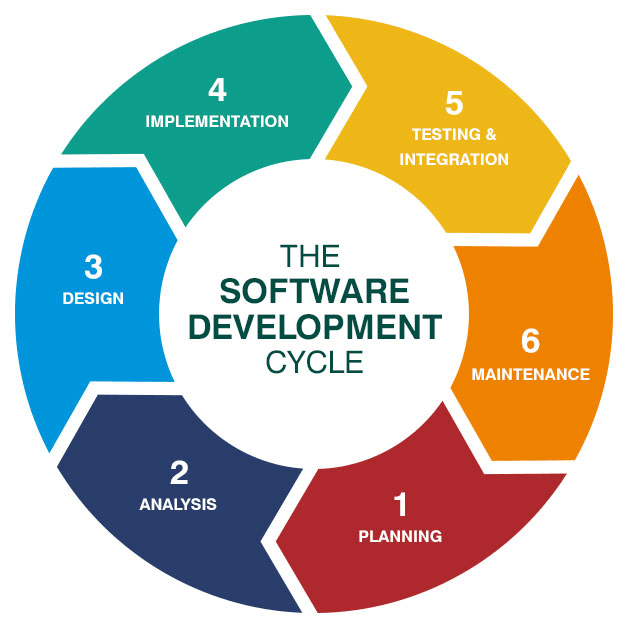
\includegraphics[width=0.6\textwidth]{pics/software_dev.png}
  \caption{Základné etapy vývoja softvéru\cite{TP:SSD}}
  \label{fig:5}
\end{figure}

Pripomíname, že obrázok je len jeden z mnohých príkladov spôsobov vývoja softvéru a viaceré zdroje uvádzajú rôzne názvy i rôzne počty fáz. My sme sa rozhodli pre nasledovnú postupnosť, čomu budú zodpovedať aj nasledujúce podkapitoly:

\begin{enumerate}
    \setlength{\itemsep}{2pt}
    \setlength{\parskip}{1pt}
    
    \item \textbf{Špecifikácia cieľov a požiadaviek}
    \item \textbf{Návrh}
    \item \textbf{Implementácia}
    \item \textbf{Overenie}
\end{enumerate}

V špecifikácii sa súčasne venujeme hĺbkovej analýze problému formou určenia konkrétnych cieľov a požiadaviek, ktoré od našej aplikácie očakávame. Častou poslednou fázou býva údžba softvéru, tú sme sa však pre dodržanie obmedzenia obsahu tejto práce rozhodli neuviesť. Ostatné fázy zodpovedajú uvedeným fázam na obrázku.

Pre prehľadné naplnenie účelov jednotlivých fáz používame v nasledujúcich podkapitolách softvérové modelovanie formou rôznych \textbf{diagramov}. Na modelovanie používame modelovací jazyk \textit{UML}, ktorý je v súčasnosti veľmi populárny a ako prostredie pre modelovanie sme sa rozhodli pre webovú stránku \textit{Visual Paradigm Online}.

Aby sme lepšie pochopili význam jazyka UML a prečo sme si ho vybrali pre náš návrh, uvádzame nasledovnú definíciu. UML (ang. Unified Modeling Language) je jazyk obsahujúci veľké množstvo nástrojov, ktoré enormným spôsobom zjednodušujú systémovú analýzu, a je dôležitým prostriedkom zlepšujúcim celkovú dizajnovú kvalitu návrhu. Používanie UML v analýze a dizajne umožňuje naplnenie systémových požiadaviek za pomoci objektovo prientovaného návrhu a modelov relačných databáz.\cite{CAVIQUE2022103569}


\subsection{Špecifikácia cieľov a požiadaviek}

Na začiatku každého procesu vývoja softvéru je vhodné jasne a prehľadne špecifikovať ciele a požiadavky na softvér - neskôr budeme sledovať ich postupné napĺňanie. Je to nutné, aby sme jasne špecifikovali a vymedzili, čo možno od našej aplikácie očakávať, čo všetko je nutné implementovať, či aký bude mať naša aplikácia dosah na bežné fungovanie užívateľa. Na všetky tieto účely slúžia rôzne typy požiadaviek, z ktorých máme viaceré uvedené v nasledovných podkapitolách.

\subsubsection*{Vyslovenie hypotézy}

Pred samotným procesom špecifikácie už konkrétnych cieľov či požiadaviek sme sa na začiatok rozhodli vysloviť akúsi stručnú hypotézu, ktorá v niekoľkých riadkoch zhrnie základné piliere našej automatizácie. Takýmto spôsobom v stručnosti zosumarizujeme všetko podstatné a budeme z tohto výroku pri neskoršom detailnejšom návrhu vychádzať, ale aj ho napĺňať a zdokonalovať. Teraz uvádzame samotnú hypotézu:

\paragraph{}

\textit{„Cieľom je vytvoriť plnohodnotnú desktopovú aplikáciu schopnú na základe poskytnutých dát o nákupe automaticky vyhľadať a stiahnuť dané položky z viacerých online letákov a na základe rôznych kritérií odporučiť najvhodnejší obchod pre nákup. Aplikácia tak bude šetriť ľudom peniaze a čas, ktoré by často minuli pri bežnom nevedomom nakupovaní.“}

\paragraph{}


Pri skúmaní vyslovenej hypotézy sa naskytuje množstvo otázok. Tak napríklad - \textit{``Aký operačný systém bude aplikácia podporovať ?"} Po dlhšej úvahe sme dospeli k nasledovnému záveru. Na základe času a prostriedkov, ktoré máme, sme sa zatiaľ rozhodli len pre podporu operačného systému Windows. To ale neznamená, že to úplne vylučujeme, zatiaľ je ale cieľom zapojiť hlavne tento systém, nakoľko je v súčasnej dobe stále najpopulárnejší. Okrem iného, máme s ním najviac skúseností.

Ďalšia, nemenej dôležitá otázka znie: \textit{``Aký programovací jazyk alebo iný nástroj v oblasti automatizácie softvéru budeme v našom návrhu využívať ?"} S touto otázkou sme sa zaoberali asi najdlhšie. Aj na základe analýzy nástrojov v predchádzajúcej kapitole sme mali možnosť rozhodnúť sa buď pre väčšie množstvo programovania, kedy by sme sa rozhodli pre realizovanie signifikantnej časti aplikácie v nejakom konkrétnom \textbf{programovacom jazyku}, alebo si zvoliť nejaký voľne dostupný \textbf{nástroj na automatizáciu}, v ktorom by programovanie nebolo až tak nutné. Po dôkladnom zvážení daných možností sme sa nakoniec rozhodli pre prvú alternatívu a programovací jazyk \textbf{Python}, a to najmä z väčších skúseností s programovaním i so samotným jazykom.

Je nutné zaoberať sa aj otázkou, \textit{aké obchody bude aplikácia podporovať ?} Odpoveď je taká, že očakávame, že systém ponúkne čo najväčšiu rôznorodosť a bude vychádzať z dostatočného množstva obchodov, a to na základe letákov dostupných online. Teda aplikácia bude schopná stiahnuť z webovej stránky aktuálne dáta predstavujúce reálne produkty ponúkané konkrétnym obchodným reťazcom v danom okamihu. V práci budeme implementovať skripty pre sťahovanie produktov zo stránky \textit{www.wolt.com}, ktorá zahŕňa viaceré reťazce fungujúce na Slovensku, ale i v zahraničí a dokonca sú tieto reťazce rozdelené aj do konkrétnych predajní.

Ostáva ešte množstvo otázok otvorených, tie sa však pokúsime zodpovedať už v samotnom návrhu. Teraz sa môžme pozrieť už na konkrétne príklady softvérových požiadaviek.
Pre lepšie pochopenie, čo to vlastne softvérové požiadavky sú, uvádzame stručnú charakteristiku. Softvérové požiadavky tvoria podstatnú časť akéhokoľvek softvérového projektu. Identifikujú a objasňujú rôzne vlastnosti a súčasti, správanie a výkon, ktorý klienti alebo užívatelia očakávajú.\cite{SB:TSR}

Softvérové požiadavky sa bežne delia nasledovne:

\begin{enumerate}
    \setlength{\itemsep}{4pt}
    \setlength{\parskip}{1pt}
    
    \item \textbf{Biznisové}
    \item \textbf{Používateľské}
    \item \textbf{Softvérové}
    \begin{enumerate}
        \item \textbf{Funkčné}
        \item \textbf{Nie-funkčné}
    \end{enumerate}
\end{enumerate}

My sa budeme zaoberať najmä biznisovými a softvérovými požiadavkami. Používateľské požiadavky nešpecifikujeme osobite formou podkapitoly, ale iba nimi dopĺňame ostatné požiadavky.

\subsubsection{Biznis požiadavky}

Biznisové požiadavky v podstate predstavujú merateľné ciele či ukazovatele projektu. Prehľadne sa pomocou nich konkretizujú dôvody, prečo sa vlastne projekt realizuje.\cite{SB:TSR} V tejto časti uvádzame niekoľko biznis požiadaviek pre náš projekt. Predstavujú našu osobnú motiváciu pre realizáciu tohto projektu.

\begin{enumerate}
    \item Aplikácia bude masívne šetriť zákazníkom čas.
    \item Aplikácia dokáže zákazníkom šetriť peniaze.
    \item Aplikácia zvýši návštevnosť jednotlivých obchodov.
    \item Systém zvýši celkovú prehľadnosť užívateľov o jednotlivých obchodoch a ich produktoch.
\end{enumerate}

Z požiadaviek vidno, že  pozitívny vplyv aplikácie na každodenné fungovanie užívateľa bude badateľný, ale takisto bude softvér prinášať pozitívny efekt aj zapojeným obchodným reťazcom.

\subsubsection{Softvérové požiadavky}

\begin{figure}[tbh]
  \centering
  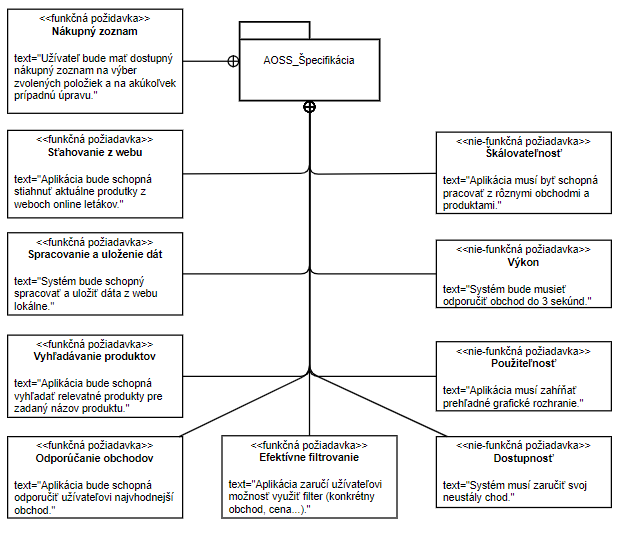
\includegraphics[width=0.8\textwidth]{pics/design/requirements_2.png}
  \caption{Softvérové požiadavky}
  \label{fig:6}
\end{figure}

Softvérové požiadavky sa ďalej delia na \textbf{funkčné} a \textbf{nie-funkčné.} Funkčné požiadavky jasne definujú, čo musí softvér vykonávať, aké sú jeho vlastnosti a funkcie. Nie-funkčné požiadavky sa sústreďujú skôr na všeobecné vlastnosti systému. Taktiež sú známe ako vlastnosti kvality.\cite{AS:FNR}

Na obrázku 3 možno vidieť niekoľko príkladov pre funkčné i nie-funkčné požiadavky charakterizujúce náš systém. Pre prehľadnosť sme sa rozhodli nezahŕňať užívateľské požiadavky osobite - na obrázku 3 sú uvedené spolu s funkčnými požiadavkami.

Z daného diagramu požiadaviek získavame lepší prehľad už aj o konkrétnych \textbf{aktéroch} či \textbf{komponentoch} nášho systému. Ak to chceme zhrnúť, systém bude musieť fungovať v nasledovnej postupnosti:

\begin{enumerate}
    \setlength{\itemsep}{4pt}
    \setlength{\parskip}{1pt}
    
    \item Sťahovať údaje z webu
    \item Spracovať a uložiť dáta
    \item Efektívne vyhľadávať produkty
    \item Inteligentne odporúčať obchody
\end{enumerate}

\subsection{Návrh riešenia}

V minulej časti sme si úspešne stanovili naše osobné biznis ciele, funkčné aj nefunkčné požiadavky na systém. Teraz sa môžme ísť venovať návrhu našej implementácii, v ktorom sa budeme pokúšať o ich postupné napĺňanie. Návrh budeme postupne rozvíjať podľa odporúčaných krokov a ilustrovať za pomoci odporúčaných diagramov.

Túto kapitolu sme sa rozhodli rozdeliť do 2 menších kapitol. Prvá z nich \ref{UCSAD} sa venuje identifikácii prípadov použitia, návrhu základnej štruktúry a architektúry v implementácii. Ďalšie z nich sa už venujú podstatným prípadom použitia, ktoré sme si identifikovali a približujú ich prúd vykonávania.


\subsubsection{Prípady použitia, štruktúra a architektúra návrhu}\label{UCSAD}

\subsubsection*{Diagram tried}\label{CD}

V tejto fáze je vhodné identifikovať jednotlivých aktérov systému, teda aké entity vystupujú a ako vzájomne spolupracujú v našej aplikácii. Na naplnenie týchto účelov sa v praxi bežne využívajú \textbf{diagramy tried}. Diagramy tried zachytávajú aspekty štruktúry softvéru, naznačujú stavebné bloky systému a aj to, ako spolu súvisia.\cite{BERGSTROM2022111413} V klasickom diagrame tried budú vystupovať \textbf{triedy} a tie budú pospájané rôznymi \textbf{vzťahmi} (šípkami) podľa toho, ako spolu súvisia.

\begin{figure}[tbh]
    \centering
    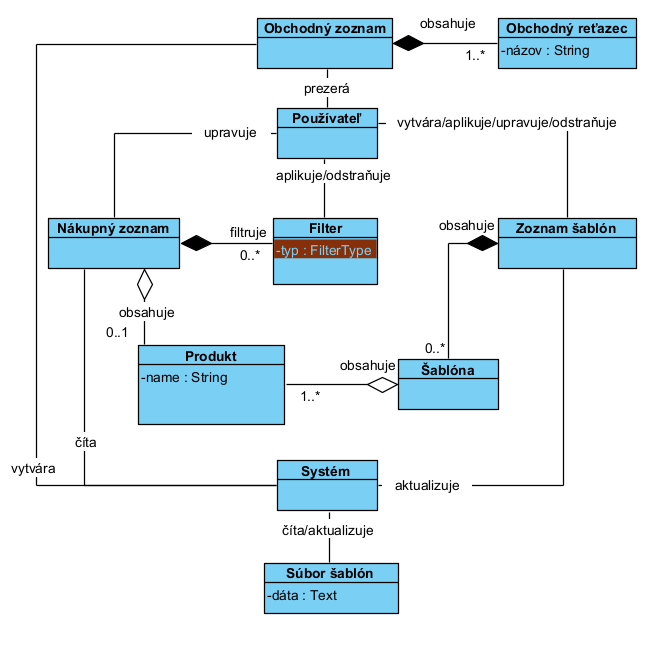
\includegraphics[width=0.8\textwidth]{pics/design/class_diagram.png}
    \caption{Diagram tried}
    \label{fig:7}
\end{figure}

Na obrázku 6 možno vidieť načrtnutú štruktúru pre našu implementáciu. Je na ňom vidieť identifikovaných niekoľko dôležitých tried i vzťahov medzi nimi. Pre prehľadnosť sme každý vzťah opísali slovne a dané slovo umiestnili bližšie k triede, ktorá má daný vzťah k druhej triede. Tak napríklad, trieda \textit{Používateľ} \textbf{upravuje} objekt triedy \textit{Nákupný zoznam}. Pre prípady vzťahov \textit{one-to-many}, teda agregovaných alebo compozičných asociacií sme uviedli aj kardinalitu. Z tejto štruktúry sa zatiaľ črtajú dvaja aktéri, a to:

\begin{enumerate}
    \item \textbf{Užívateľ} (User)
    \item \textbf{Systém} (System)
\end{enumerate}


Začnime opisom funkcionality pre bežného užívateľa aplikácie. Možno vidieť, že trieda s názvom \textit{User} môže vykonávať celkovo štyri funkcie. Prvá z nich umožňuje užívateľovi upravovať svoj nákupný zoznam podľa potreby. To zahŕňa pridávanie konkrétnych objektov pre triedu \textit{Product}, kde užívateľ uvedie názov produktu a pridá ho do svojho zoznamu. Užívateľ takisto môže zo zoznamu produkt odstrániť. Rovnako tak môže aplikovať filter, či už na filtrovanie nákupov podľa názvu obchodu alebo ceny. Užívateľ takisto dokáže upravovať svoj vlastný zoznam šablón. Šablóny sme si už popísali a používateľ ich teda môže vytvárať, prezerať či odtraňovať. Vždy má dostupný aktualizovaný zoznam šablón. Na záver má užívateľ takisto možnosť prezerať si zoznam reťazcov odporúčaných aplikáciou.

Teraz sa presuňme na funkcie samotného systému. Pri štarte aplikácie systém číta externý súbor obsahujúci dáta týkajúce sa šablón pre konkrétneho užívateľa. Z týchto dát vytvorí zoznam, ktorý naplní špecifickými objektmi triedy \textit{Šablóna} a ktorý je počas behu programu plne sprístupnený užívateľovi. Elementy tohto zoznamu sú počas behu programu pravidelne aktualizované, aby v prípade pádu alebo inej nečakanej udalosti dochádzalo k čo najmenším stratám na dátach. Systém počas programu v prípade potvrdenia užívateľom číta objekt triedy \textit{Nákupný zoznam}, z ktorého následne stiahne požadované dáta z viacerých webových stránok predstavujúcich online letáky. Tieto dáta následne vyhodnotí a poskytne užívateľovi objekt triedy \textit{Obchodný zoznam}, ktorý predstavuje jeden alebo viac odporúčaných reťazcov.

Na úspešné vyhodnotenie užívateľských požiadaviek musí systém stiahnúť dáta z viacerých webových stránok, porovnať ich a odporučiť najlepšie prípady. Bolo by teda vhodné pridať do diagramu aj nejakú triedu predstavujúcu takúto stránku, to sme však pre celkovú prehľadnosť diagramu neuvádzali.

\subsubsection*{Diagram prípadov použitia}\label{DESIGN:UCD}

Počas fázy analýzy požiadaviek, diagramy prípadov použitia pomáhajú identifikovať aktérov a pomocou prípadov použitia definovať správanie sa systému. Okrem aktérov a prípadov použitia UML definuje menšie množstvo možných vzťahov na nadviazanie štruktúry medzi aktérmi a prípadmi použitia:

\begin{enumerate}
    \item \textbf{Association}
    \item \textbf{Extend}
    \item \textbf{Include}
    \item \textbf{Generalization}
\end{enumerate}

Prvý vzťah predstavuje najbežnejší vzťah medzi prípadmi použitia a aktérmi a naznačuje asociáciu. Často to znamená, že aktér vykonáva daný prípad. Ďalší zo vzťahov hovorí, že jeden prípad použitia môže byť rozšírený o iný za splnenia určitej podmienky. Tretí znamená, že jeden prípad použitia v určitom momente zahŕňa a vykonáva iný prípad použitia. Posledný vzťah znamená, že jeden prípad generealizuje, teda špecifikuje, rodičovský prípad. Podobne, ako fungujú princípy OOP, detský prípad dedí všetky vlastnosti a asocácie rodiča.\cite{von2002modeling}

\begin{figure}[tbh]
    \centering
    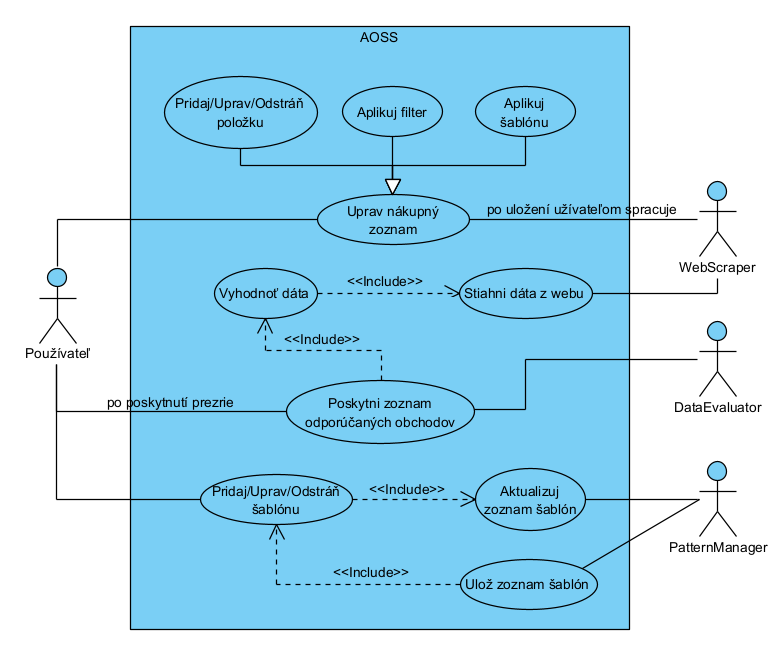
\includegraphics[width=0.9\textwidth]{pics/design/use_case_diag.png}
    \caption{Diagram prípadov použitia}
    \label{fig:8}
\end{figure}

Obrázok 7 zobrazuje náš vlastný diagram prípadov použitia. Prvé, čo je dobré si všimnúť, je modrý štvoruholník predstavujúci oblasť pôsobnosti systému. Obsahuje názov aplikácie a možné prípady použitia, ktoré jednotliví aktéri vykonávajú.\cite{von2002modeling}

V diagrame tried v kapitole \ref{CD} sme už aktérov v systéme ako tak načrtli, boli to triedy \textit{Používateľ} a \textit{Systém}. Aktér \textbf{Používateľ} predstavuje bežného užívateľa našej aplikácie. Užívateľia systémov sú v diagramoch prípadov použitia bežne umiestňovaní na ľavú stranu.  Systém predstavuje už spomínaná oblasť pôsobenia a každý prípad použitia by mal byť asociovaný s nejakým konkrétnym aktérom, preto sme identifikovali celkovo troch aktérov, ktorí predstavujú \textbf{komponenty} systému.

Ako vieme, diagram prípadov použitia takisto abstraktne definuje funkcionalitu systému. Z obrázka vidno, že bežnému užívateľovi systém umožňuje upravovať nákupný zoznam, a to či už aktualizáciou položiek predstavujúce produkty v obchode alebo aplikovaním nejakého typu filtra na zoznam. Takisto v prípade opakovaného nákupu môže využiť aj nejakú z predefinovaných šablón. V prípade šablón systém takisto umožňuje užívateľovi aktualizovať svoj vlastný zoznam šablón. Posledný prípad použitia predstavuje funkciu systému, ktorá užívateľovi prehľadne zobrazí odporúčané obchodné reťazce.

Čo sa týka samotných funkcií systému a jeho komponentov, tak už vieme, že systém musí vedieť na základe nákupného zoznamu, ktorý si užívateľ špecifikoval, stiahnuť potrebné dáta z podporovaných online letákov. Táto funkcionalita náleží komponentu \textit{WebScraper}. Komponent \textit{DataEvaluator} predstavuje akýsi algoritmus, ktorý stiahnuté dáta z webu vyhodnotí a poskytne mieru uspokojenia pre jednotlivé obchodné reťazce. V diagrame si možno všimnúť, že nato, aby bol užívateľov poskytnutý zoznam odporúčaných obchodov, je potrebné najskôr vyhodnotiť dáta. Nato je zase potrebné stiahnuť dáta z webu. Všetky tieto typy asociácie predstavujú vzťah \textit{$<<$include$>>$}. Posledný komponent \textit{PatternManager} má na starosti pravidelnú aktualizáciu užívateľmi definovaných šablón počas behu programu. V diagrame si možno opäť všimnúť, že nato, aby užívateľ mohol pracovať s zoznam šablón sa vyžaduje, aby bol vykonaný prípad použitia \textit{Načítaj zoznam šablón}. Takisto, aby mohol byť vykonaný prípad ulož zoznam šablón je potrebná nejaká modifikácia zo strany používateľa.

\subsubsection{Sťahovanie dát z online letákov}

V diagrame prípadov použitia sme si definovali dva významné prípady použitia \textit{Stiahni dáta z webu} a \textit{Poskytni zoznam odporúčaných obchodov}. Oba totižto predstavujú vcelku veľkú implementačnú výzvu, a  preto pre ne poskytneme podrobnejší návrh v nasledovných dvoch podkapitolách. Začnime prvým z nich - ako už názov napovedá, bude úlohou aktéra systému \textit{WebScraper} poslať žiadosť na online web stránku, ktorá mu ako odpoveď vráti svoje dáta. V našom prípade pôjde o online webový leták nejakého obchodného reťazca, odkiaľ budeme sťahovať dáta relevatné pre jednotlivé produkty. Toto je nutné z toho dôvodu, aby naša aplikácia bola schopná porovnávať čo najaktuálnejšie výsledky jednotlivých reťazcov.

Teraz sa môžme presunúť na trochu detailnejší návrh vyššie opísaných požiadaviek pomocou \textbf{diagramov sekvencií}. Pre správne pochopenie voľby práve tohto typu diagramu uvádzame stručnú definíciu - sekvenčné diagramy reprezentujú interakcie vykonávajúce sa sekvenčne medzi jednotlivými komponentami v softvérovej architektúre a rovnako aj ich aktívny čas.\cite{KARAMPURE2021457} Tento diagram je v tomto prípade veľmi vhodný, pretože nám vo väčších detailoch priblíží interakciu jednotlivých komponentov systému a aj ich čas.

Na obrázku 8 možno vidieť náš vlastný diagram sekvencií opisujúci prípad použitia \textit{Stiahni dáta z webu}. Celkovo sme si v ňom definovali 4 entity, jedna predstavuje \textbf{externého používateľa} aplikácie a ostatné sú \textbf{objekty} alebo \textbf{komponenty systému}. Keď si priblížime dané komponenty, tak \textit{DataManager} a \textit{WebScraper} budú tvoriť náš vlastný systém, resp. aplikáciu. \textit{Online Web Leták} predstavuje externú web stránku, teda komponent systému konkrétneho reťazca.

Samotné \textbf{interakcie} sú reprezentované šípkami. Z obrázku vidno, že užívateľ si vyžiada dáta o produkte, teda si vytvorí nákupný zoznam a pošle ho aplikácií na vyhodnotenie. Komponent \textit{DataManager} obdrží dané požiadavky, no najskôr skontroluje, či nie je nutné aktualizovať dáta uložené lokálne. Tu nastáva možnosť, že dáta nie sú aktuálne a je najskôr potrebné stiahnúť nové. V takom prípade vyšle žiadosť komponentu \textit{WebScraper} obsahujúcu názov žiadaného produktu. \textit{WebScraper} najskôr musí cez internet nadviazať spojenie s online letákom pomocou \textbf{protokolu HTTP}. Prvým krokom je HTTP žiadosť, ktorá bude zahŕňať:

\begin{enumerate}
    \item \textbf{Unikátny zdrojový lokátor - URL}
    \item \textbf{Autorizačný kľúč}
\end{enumerate} 

Formát samotného URL bude samozrejme závislý na formáte URL webovej stránky online letáku a bude zahŕňať samotný názov produktu, pre ktorý sa na stránke zobrazia dostupné výsledky. Rovnako bude obsahovať aj číslo webovej stránky, ak bude informácií o produktoch príliš veľa, aby boli len na jednej stránke. Autorizačný kľúč slúži na autorizáciu žiadosti nášho systému o dáta spočívajúcu v potvrdení, že nejde o nejakého robota, ktorý chce vykonávať pravidelné sťahovanie dát, nakoľko v súčasnosti má veľké množstvo  webových stránok zabudované rôzne obranné mechanizmy proti takýmto pokusom.

Ak je autorizácia úspešná a spojenie nadviazané, pošle webová stránka \textbf{HTTP odpoveď}, ktorá bude obsahovať dáta v jazyku \textit{HTML}. Takéto dáta sú zvyčajne veľmi robustné a bude úlohou komponentu \textit{WebScraper} ich spracovať a extrahovať z nich to najpodstatnejšie, a to názvy produktov a ich ceny. Proces extrakcie bude opäť závislý na štruktúry konkrétnej stránky.

Po úspešnom stiahnutí a spracovaní dát z webu má \textit{WebScraper} ešte za úlohu dáta niekde uložiť. Tu sa naskytá veľa možností, napríklad uložiť dáta lokálne do súboru, prípadne do databázy. Pre jednoduchosť našej práce sme sa rozhodli pre ukladanie do súboru vo formáte \textbf{csv}. To znamená, že v jednotlivých riadkoch v súbore budú atribúty (názov, cena...) oddelené čiarkou.

\begin{figure}[tbh]
    \centering
    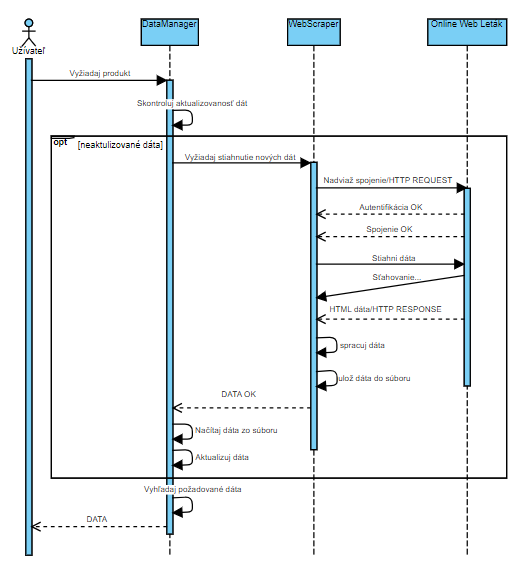
\includegraphics[width=0.7\textwidth]{pics/design/web_scraping.png}
    \caption{Sekvenčný diagram pre PP \textit{Stiahni dáta z webu}}
    \label{fig:9}
\end{figure}

To, čo komponent \textit{DataManager} spraví s danými dátami, závisí od konkrétneho prípadu. Ak užívateľ požaduje iba vyhľadanie nejakého lokálneho produktu, tak iba vyhľadá spomedzi lokálnych dát tie relevatné pre požadovaný produkt. Ak však užívateľ požaduje automatické odporučenie konkrétneho reťazca, tak komponent musí pomocou algoritmu vyhľadať produkty vo všetkých reťazcoch a z nich na základe kritéria nájsť tie najvhodnejšie.

Len pripomíname, že v diagrame nie je pre prehľadnosť zahrnuté \textbf{grafické rozhranie}, cez ktoré komunikuje užívateľ so systémom a jeho komponentami.

\subsubsection{Efektívne vyhľadávanie produktov a odporúčanie reťazcov}

V minulej časti sme podrobne navrhli, ako budeme schopní stiahnuť reálne a aktuálne dáta dostupné z online letákov jednotlivých reťazcov. Takisto sme opísali ako ďalej dané dáta spracujeme a uložíme. Teraz sa pôjdeme pozrieť na ďalšie dva dôležité prvky našej aplikácie, a to je efektívne vyhľadávanie relevantných produktov a inteligentné odporúčanie reťazcov na základe definovaných metrík. Na naplnenie týchto cieľov bude nutná realizácia určitých algoritmov, preto v nasledujúcich podkapitolách uvádzame detailnejší opis ich jednotlivých krokov pomocou \textbf{diagramov aktivít}. 

Diagram aktivití sú v UML grafické notácie opisujúce správanie inštancií tried počas ich životnosti. Často slúžia na modelovanie toku systému v modelovaní softvérových či webových aplikácií, prípadne v biznis modelovaní.\cite{ABBAS2021101911}


Konkrétne v našom prípade  pôjde o to, že užívateľ si buď vyhľadá produkt alebo vytvorí svoj vlastný nákupný zoznam, na ktorý bude očakávať automatizované spracovanie, vyhodnotenie a odporučenie obchodného najvýhodnejšieho obchodného reťazca. Je teda nutné implementovať nejaký vysoko efektívny a optimalizovaný algoritmus na vyhľadávanie spomedzi desaťtisícov možných produktov a hľadanie najväčšej zhody s hľadanou položkou.

Na hľadanie zhody medzi textovými reťazcami existujú viaceré algoritmy, my sme sa rozhodli pre \textbf{Levenshtein-ovu vzialenosť}.

Levenshtein-ova vzdialenosť je metrika mejarúca počet operácií (vloženie, odstránenie alebo nahradenie znaku) požadovaných na konvertovanie reťazca znakov A na reťazec B. Používa sa v rôznych výpočtových doménach, zahŕňajúc textovú či hudobnú analýzu, prípadne v informatike.\cite{CASTELLSRUFAS2023103019}

\subsubsection*{PP04 - Nájdi zhodu medzi produktami}

Teraz sa môžme ísť detailnejšie pozrieť na spomínaný prípad použitia identifikovania zhody medzi hľadaným produktom a dostupnými produktami pre jednotlivé reťazce. Z diagramu prípadov použitia uvedeného v kapitole \ref{DESIGN:UCD} už vieme, že ho vykonáva entita \textit{DataManager}. 
Tento prípad použitia a jeho kroky sme opísali pomocou diagramu aktivít na obrázku 9 nižšie.

Diagram používa tzv. "plávacie línie" (ang. \textit{swimlanes}) pre identifikáciu účinkujúcich v a nimi vykonávaných aktivít v diagrame. Celkovo sa na tejto interakcií podielajú dve entity:

\begin{enumerate}
    \item \textbf{Užívateľ}
    \item \textbf{DataManager}
\end{enumerate}

Ako sme už spomínali, proces začne užívateľ, ktorý si napríklad vytvorí nákupný zoznam a potvrdí svoj výber. Následne je nutné požiadavku spracovať, a to tak, že entita \textit{DataManager} načíta prvú položku. Začne sa vykonávať dôležitá aktivita \textit{Najdi zhodu medzi produktami}, ktorá dostane na vstup spracovávanú položku, plus dostupné dáta, ktoré predstavujú uložené produkty v súboroch. Pre každý dostupný produkt poskytovaný nejakým reťazcom je nutné identifikovať zhodu pomocou Levenshtein-ovej vzdialenosti a tú uložiť do \textbf{výstupného súboru}. Toto sa opakuje, dokým nie sú všetky produkty vybavené.

Z diagramu vidno, že proces končí na strane enitity \textit{DataManager}. Tá spracovala užívateľovu požiadavku o vyhľadanie položky (prípadne celého zoznamu) a dané zistenia uložila do súboru. Tieto dáta môže ďalej spracovať entita \textit{ShopSearcher}, ktorému sa budeme venovať v nasledujúcej kapitole.

\begin{figure}[tbh]
    \centering
    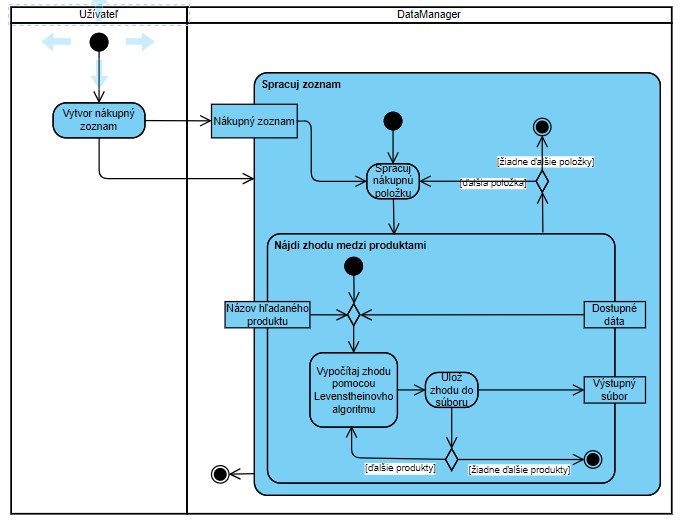
\includegraphics[width=0.8\textwidth]{pics/design/data_search.png}
    \caption{Diagram aktivít pre PP04 \textit{Nájdi zhodu medzi produktami}}
    \label{fig:10}
\end{figure}

\subsubsection*{PP05 - Odporuč najvhodnejší reťazec}

Entita \textit{DataManager} úspešne identifikovala zhody pre všetky produkty v zozname so všetkými dostupnými produktami. Na základe týchto dát teraz entita \textit{ShopSearcher} vyhodnotí dané zhody a na základe kritérií užívateľa odporučí ten najvhodnejší reťazec (prípadne reťazce). Detailnejšie si to opíšeme pomocou diagramu uvedenom na obrázku 10. Tu máme 3 aktérov, a to používateľa a entity \textit{DataManager} a \textit{ShopSearcher}. Keď sa pozrieme na prvé dve aktivity, vidíme, že ide o tie, ktoré sú detailnejšie opísané v predchádzajúcom diagrame. Toto naznačuje významné logické nadväzovanie diagramov a interakcie medzi entitami.

Teraz sa poďme bližšie pozrieť na prípad použitia \textit{Odporuč najvhodnejší reťazec}. Ten na vstup dostane relevantné produkty spracované \textit{DataManager} entitou a bude postupne pre každý reťazec počítať jeho \textit{mieru celkovej úspešnosti}. Pre každý reťazec sa najskôr extrahujú relevantné produkty ponúkané daným reťazcom a to sa ešte rozdelí na zhody na základe konkrétneho produktu. Entita \textit{DataManager} teda bude musieť identifikovať obchod aj konkrétnu skupinu relevantných produktov pre špecifický produkt z nákupného zoznamu pomocou \textbf{unikátnych identifikátorov}.

Ak sa stane, že bude viacero relevantných produktov pre hľadaný produkt, bude užívateľ vyzvaný, aby určil, ktoré sú preňho potrebné. Cieľom nášho projektu je ale aplikácia slúžiaca ako automatizácia, a preto bude našou snahou, aby nevznikali viaceré zhody na jeden produkt.

Keď budú všetky produkty pre daný reťazec úspešne spracované, je nutné vypočítať dve metriky:

\begin{enumerate}
    \item Miera produktovej dostupnosti
    \item Celková cena
\end{enumerate}

Produktová dostupnosť predstavuje percento uspokojených produktov z nákupného zoznamu. Celková cena bude predstavovať súčet cien všetkých produktov v zozname vytvorenom entitou \textit{ShopSearcher}. Užívateľ má možnosť pri vytváraní zoznamu definovať vlastné kritéria, teda napríklad či chce viac mieru produktovej dostupnosti alebo ceny. Entita \textit{ShopSearcher} teda pre každý reťazec vypočíta jeho \textbf{celkovú úspešnosť} na základe produktovej dostupnosti a jej váhy a ceny a jej váhy.

\begin{figure}[tbh]
    \centering
    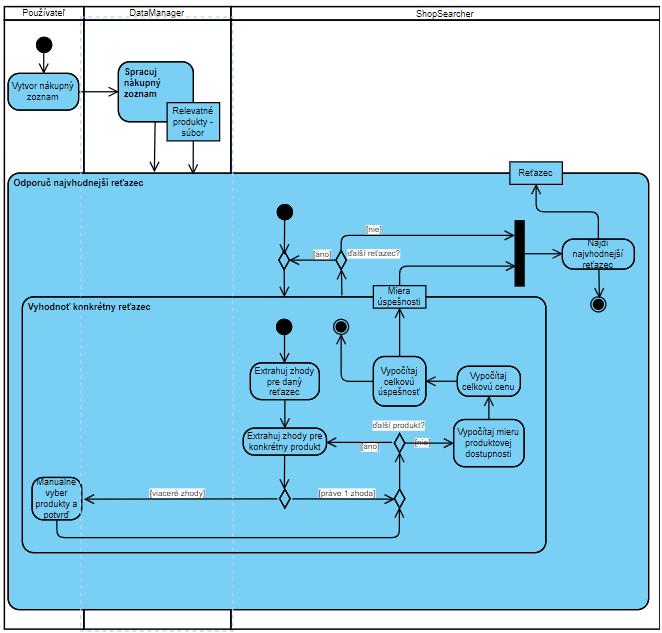
\includegraphics[width=0.9\textwidth]{pics/design/intelligent_shop_search.png}
    \caption{Diagram aktivít pre PP05 \textit{Odporuč najvhodnejší reťazec}}
    \label{fig:11}
\end{figure}


\subsection{Implementácia}

\subsection{Overenie}

\newpage

\section {Zhodnotenie výsledkov}



\newpage

\section {Technická dokumentácia}


\newpage



\bibliography{literatura}
\bibliographystyle{ieeetr}



%\vspace*{0cm}

%\author{Filip Mojto}
%\title{Your Title}
%\date{October 2023}



% Set up the upper part of the first page
%\newgeometry{top=2cm} % Adjust the top margin as needed
%\maketitle % Title and author information
%\vspace*{1cm} % Add vertical space

%Your text in the upper part of the first page.

% Restore the standard page layout
%\restoregeometry



%\maketitle

%\section{Introduction}

\end{document}
